\documentclass[tikz, border=10pt]{standalone}
\usetikzlibrary{arrows.meta, positioning, shapes, calc}

\usepackage[T1]{fontenc}
\usepackage{lmodern}
\begin{document}
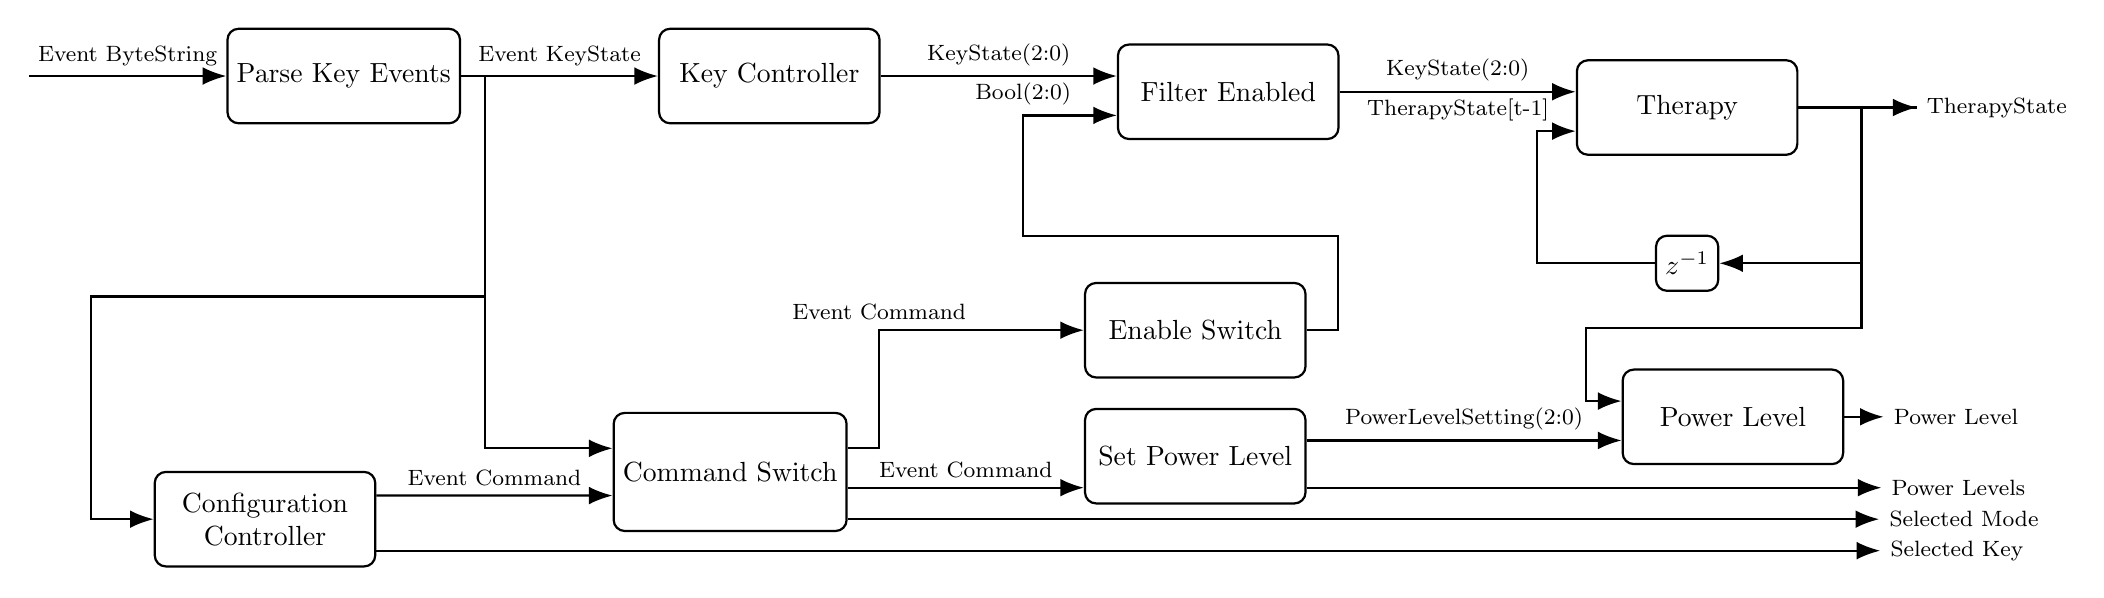
\begin{tikzpicture}[
  block/.style = {draw, thick, minimum width=2.8cm, minimum height=1.2cm, align=center, rounded corners},
  sum/.style = {draw, circle, inner sep=1pt, minimum size=6mm, node contents={+}},
  line/.style = {thick, -{Latex[length=3mm]}},
  signal/.style = {font=\footnotesize, midway, above},
  signalbelow/.style = {font=\footnotesize, midway, below}
]

  % Nodes
  \node[block] (parser) {Parse Key Events};
  \node[block, right=2.5cm of parser] (controller) {Key Controller};
  \node[block, right=3cm of controller, yshift=-0.2cm] (filterenabled) {Filter Enabled};
  \node[block, right=3cm of filterenabled, yshift=-0.2cm] (therapy) {Therapy};
  \node[block, minimum size=7mm, below=1cm of therapy] (delay) {$z^{-1}$};
  \node[block, below=4.4cm of parser, xshift=-1cm] (configuration) {Configuration\\Controller};
  \node[block, right=3cm of configuration, yshift=0.6cm, minimum height=1.5cm] (commandswitch) {Command Switch};
  \node[block, right=3cm of commandswitch, yshift=1.8cm] (setenabled) {Enable Switch};
  \node[block, right=3cm of commandswitch, yshift=0.2cm] (setpowerlevel) {Set Power Level};
  \node[block, right=4cm of setpowerlevel, yshift=0.5cm] (powerlevel) {Power Level};

  % Connections
  \draw[line] (-4,0) -- (parser.west) node[signal]{Event ByteString};
  \draw[line] (parser.east) -- node[signal]{Event KeyState} (controller.west);

  % Controller -> Filter -> Therapy
  \draw[line] (controller.east) -- node[signal]{KeyState(2:0)} ([yshift=0.2cm]filterenabled.west);
  \draw[line] (filterenabled.east) -- node[signal]{KeyState(2:0)} ([yshift=0.2cm]therapy.west);

  % Therapy output
  \draw[line] (therapy.east) -- ++(1.5,0) coordinate (out) node[right, font=\footnotesize]{TherapyState};

  % Feedback path through delay
  \draw[line] (out) -- ++(-0.7,0)|- (delay.east);
  \draw[line] (delay.west) -| ++(-1.5,1.5) |- ([yshift=-0.3cm]therapy.west) node[signal, above, xshift=-1cm]{TherapyState[t-1]};

  % Stage 2
  \draw[line] ([xshift=0.3cm]parser.east) -- ++(0,-2.8) |- ++(-5,0) |- (configuration.west);
  \draw[line] ([yshift=0.3cm]configuration.east) -- node[signal]{Event Command} ([yshift=-0.3cm]commandswitch.west);
  \draw[line] ([yshift=0.2cm]setpowerlevel.east) -- node[signal]{PowerLevelSetting(2:0)} ([yshift=-0.3cm]powerlevel.west);
  \draw[line] ([yshift=-0.4cm]setpowerlevel.east) -- ++(7.3,0) node[right, font=\footnotesize]{Power Levels};
  \draw[line] ([xshift=-0.7cm]out) -- ++(0,-2.8) |- ++(-3.5,0) |- ([yshift=0.2cm]powerlevel.west);
  \draw[line] (powerlevel.east) -- ++(0.5,0) node[right, font=\footnotesize]{Power Level};
  \draw[line] ([yshift=-0.4cm]configuration.east) -- ++(19.1,0) node[right, font=\footnotesize]{Selected Key};

  % Stage 3
  \draw[line] ([yshift=-0.2cm]commandswitch.east) -- node[signal]{Event Command} ([yshift=-0.4cm]setpowerlevel.west);
  \draw[line] ([yshift=-0.6cm]commandswitch.east) -- ++(13.1,0) node[right, font=\footnotesize]{Selected Mode};
  \draw[line] ([yshift=0.3cm]commandswitch.east) -- ++(0.4,0) -| ++(0,1.4) |- node[signal]{Event Command} (setenabled.west);
  \draw[line] (setenabled.east) -- ++(0.4,0) -| ++(0,1.2) -| ++(-4,0) |- node[signal]{Bool(2:0)} ([yshift=-0.3cm]filterenabled.west);
  \draw[line] ([xshift=0.3cm]parser.east) |- ([yshift=0.3cm]commandswitch.west);

\end{tikzpicture}
\end{document}
